\subsubsection{交集}

已知6的正约数的集合为$$A = \{1, 2, 3, 6\}\text{,}$$
10的正约数的集合为$$B=\{1, 2, 5, 10\}\text{,}$$
那么6与10的正公约数的集合为$$\{1, 2\}\text{。}$$

容易看出,集合$\{1, 2\}$是由所有属于$A$且属于$B$的元素(即$A$,$B$的公共元素)所组成的。


\begin{wrapfigure}[10]{r}{5.8cm}
    \centering
    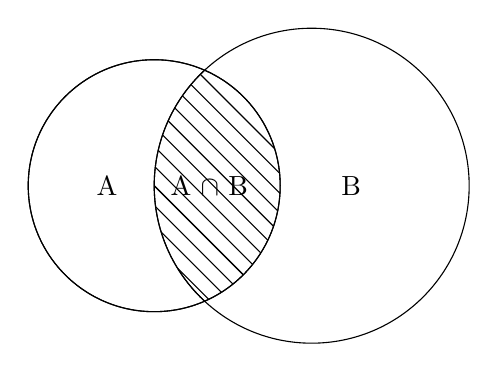
\begin{tikzpicture}
        \node at (-0.6, 0) {A};
        \node at (0.7, 0) {A $\cap$ B};
        \node at (2.5, 0) {B};
        \draw (0, 0) circle [radius=1.6];
        \draw (2, 0) circle [radius=2];
        \clip[draw] (0,0) circle [radius=1.6];
        \clip[draw] (2,0) circle [radius=2];
        \foreach \x in {-0.75,-0.5,-0.25,0,0,0.25,0.5,0.75,1,1.25,1.5,1.75,2}
        \draw[xshift=\x cm]  (-2,2)--(2,-2);
    \end{tikzpicture}
    \vspace{-10pt}
    \caption{}\label{fig:1-2}
\end{wrapfigure}

一般地,由所有属于集合$A$且属于集合$B$的元素所组成的集合,叫做$A$,$B$的\textbf{交集},记作$A \cap B$(可读作“$A$交$B$”),即
$$A \cap B = \{x \mid x \in A \text{,且} x \in B\} \text{。}$$

这样,6与10的正公约数的集合,可以从求6的正约数的集合与10的正约数的集合的交集而得到,即
$$\{1, 2, 3, 6\} \cap \{1, 2, 5, 10\} = \{1, 2\} \text{。}$$

图 \ref{fig:1-2} 中的阴影部分,表示集合$A$,$B$的交集$A \cap B$。

由交集定义容易推出,对于任何集合$A$,$B$,有
\begin{gather*} 
    A \cap A = A, \quad A \cap \kongji = \kongji , \\
    A \cap B = B \cap A \text{。}
\end{gather*}

\liti 设 $A=\{x \mid x>-2\}$, $B=\{x \mid x<3\}$,求$A \cap B$。

\jie
\begin{minipage}[t]{7cm}
    \gongshishangyi
    \begin{align*}
        A \cap B &= \{x \mid x>-2\} \cap \{x \mid x<3\} \\
                 &= \{x \mid -2<x<3\} \text{。} \\
    \end{align*}
\end{minipage}

\liti 设 $A=\{(x,y) \mid 4x+y=6\}$, $B=\{(x, y) \mid 3x+2y=7\}$,求$A \cap B$。

\jie
\begin{minipage}[t]{10cm}
    \gongshishangyi
    \begin{align*}
        A \cap B &= \{(x,y) \mid 4x+y=6\} \cap \{(x, y) \mid 3x+2y=7\} \\
                 &= \left\{ (x,y) \,\middle|\, \begin{cases}
                    4x + y &= 6,\\
                    3x + 2y &= 7
                 \end{cases} \quad \right\}\\
                 &= \{(1,2)\} \text{。} \\
    \end{align*}
\end{minipage}

\liti 设 $A =\{\text{等腰三角形}\}$,$B=\{\text{直角三角形}\}$,求$A \cap B$。

\jie
\begin{minipage}[t]{10cm}
    \gongshishangyi
    \begin{align*}
        A \cap B &= \{\text{等腰三角形}\} \cap \{\text{直角三角形}\} \\
                 &= \{\text{有两边相等且有一个角是直角的三角形}\} \\
                 &= \{\text{等腰直角三角形}\} \text{。}
    \end{align*}
\end{minipage}

形如 $2n\ (n \in Z)$的整数叫做\textbf{偶数},形如$2n+1\ (n \in Z)$的整数叫做\textbf{奇数}。全体奇数的集合简称\textbf{奇数集},全体偶数的集合简称\textbf{偶数集}。我们再看一个例子。

\liti 已知$A$为奇数集,$B$为偶数集,$Z$为整数集,求$A \cap Z$,$B \cap Z$,$A \cap B$。

\jie 
\begin{minipage}[t]{8cm}
    \gongshishangyi
    \begin{gather*}
        A \cap Z = \{\text{奇数}\} \cap \{\text{整数}\} = \{\text{奇数}\} = A , \\
        B \cap Z = \{\text{偶数}\} \cap \{\text{整数}\} = \{\text{偶数}\} = B , \\
        A \cap B = \{\text{奇数}\} \cap \{\text{偶数}\} = \kongji \text{。}
    \end{gather*}
\end{minipage}

\lianxi

\begin{xiaotis}

\begin{wrapfigure}{R}{3.6cm}
    \centering
    \vspace{-8em}
    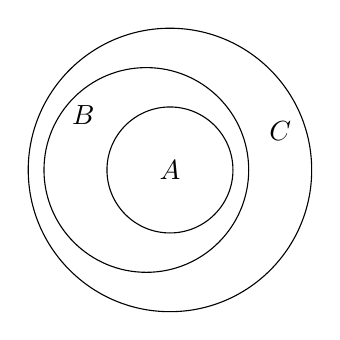
\begin{tikzpicture}
        \draw (0, 0) circle [radius=0.8];
        \draw (-0.3, 0) circle [radius=1.3];
        \draw (0, 0) circle [radius=1.8];
        \node at (0, 0) {$A$};
        \node at (-1.1, 0.7) {$B$};
        \node at (1.4, 0.5) {$C$};
    \end{tikzpicture}
    \vspace{-10pt}
    \caption*{(第1题)}\label{fig:ex1-2-1}
\end{wrapfigure}

\xiaoti{图中$A$,$B$,$C$表示集合,说明它们之间有什么包含关系。}

\xiaoti{写出集合$\{a, b, c\}$的所有子集及真子集。}

\xiaoti{用适当的符号($\in$,$\not \in$,$=$,$\subset$,$\supset$)}填空:

\begin{xiaoxiaotis}
    \begin{tabular}[t]{*{2}{@{}p{14em}}} 
        \xiaoxiaoti {$a \xhx \{a\}$;} & \xiaoxiaoti {$a \xhx \{a,b,c\}$;} \\
        \xiaoxiaoti {$d \xhx \{a,b,c\}$;} & \xiaoxiaoti {$\{a\} \xhx \{a,b,c\}$;} \\
        \xiaoxiaoti {$\{a,b\} \xhx \{b,a\}$;} & \xiaoxiaoti {$\{3,5\} \xhx \{1,3,5,7\}$;} \\
        \xiaoxiaoti {$\{2,4,5,8\} \xhx \{2,8\}$;} & \xiaoxiaoti {$\kongji \xhx \{1,2,3\}$;}
    \end{tabular}
\end{xiaoxiaotis}

\xiaoti{写出方程 $x+3=\dfrac{x}{2} - 5$的解集并进行化简。}

\xiaoti{写出方程组
$$
\begin{cases}
    2x + 3y &= 1,\\
    3x - 2y &= 3
\end{cases}
$$
的解集并进行化简。
}

\xiaoti{写出不等式$3x+2<4x-1$的解集并进行化简。}

\begin{figure}[htbp]
    \centering
    \begin{minipage}{7cm}
    \centering
    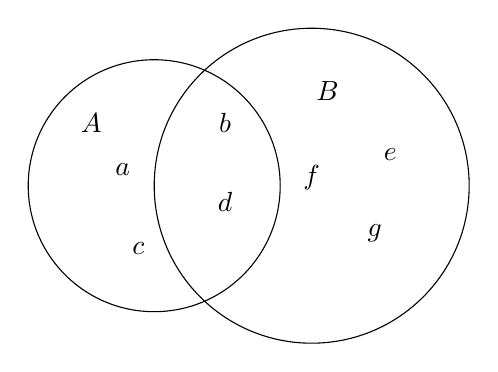
\begin{tikzpicture}
        \draw (0, 0) circle [radius=1.6];
        \draw (2, 0) circle [radius=2];
        \node at (-0.8, 0.8) {$A$};
        \node at (2.2, 1.2) {$B$};
        \node at (-0.4, 0.2) {$a$};
        \node at (0.9, 0.8) {$b$};
        \node at (-0.2, -0.8) {$c$};
        \node at (0.9, -0.2) {$d$};
        \node at (3, 0.4) {$e$};
        \node at (2, 0.1) {$f$};
        \node at (2.8, -0.6) {$g$};
    \end{tikzpicture}
    \caption*{(第7题)}\label{fig:ex1-2-7}
    \end{minipage}
    \qquad
    \begin{minipage}{6cm}
    \centering
    \begin{tikzpicture}
        \coordinate (G) at (0,0);
        \coordinate (B) at (1.6,0);
        \coordinate (A) at ($(G)!1.0!120:(B)$);
        \coordinate (C) at ($(G)!1.0!240:(B)$);
    
        \draw (A) circle (1.6);
        \draw (B) circle (1.6);
        \draw (C) circle (1.6);
        \node at (A) {$A$};
        \node at (B) {$B$};
        \node at (C) {$C$};
    
        \begin{scope}
            \clip (A) circle (1.6);
            \clip (B) circle (1.6);
            \foreach \x in {1.25,1.5,1.75,2,2.25,2.5,2.75,3,3.25,3.5}
            \draw[xshift=\x cm]  (-4,2)--(2,-2);
        \end{scope}
    
        \begin{scope}
            \clip (A) circle (1.6);
            \clip (C) circle (1.6);
            \foreach \x in {-0.5,-0.25,0,0,0.25,0.5,0.75}
            \draw[xshift=\x cm]  (-4,2)--(2,-2);
        \end{scope}
    
        \begin{scope}
            \clip (B) circle (1.6);
            \clip (C) circle (1.6);
            \foreach \x in {0,0.25,0.5,0.75,1}
            \draw[xshift=\x cm]  (-4,2)--(2,-2);
        \end{scope}
    \end{tikzpicture}
    \caption*{(第8题)}\label{fig:ex1-2-8}
    \end{minipage}
\end{figure}

\xiaoti{如图,设 $A=\{a,b,c,d\}$, $B=\{b,d,e,f,g\}$。}

\begin{xiaoxiaotis}
    \xiaoxiaoti{求 $A \cap B$,$B \cap A$;}

    \xiaoxiaoti{用适当的符号($\supset$,$\subset$,$=$)填空:\\
        \twoInLine{$A \cap B \xhx A$,}{$A \cap B \xhx B \cap A$,} \\
        \twoInLine{$B \xhx A \cap B$,}{$\kongji \xhx B \cap A$。}
    }

\end{xiaoxiaotis}


\xiaoti{图中$A$,$B$,$C$表示集合,把各个阴影部分所表示的集合分别标出来,并用适当的符号表示它们同$A$,$B$,$C$之间的包含关系。}

\xiaoti{设 $A = \{x \mid x<5\}$, $B = \{x \mid x \ge 0\}$,求 $A \cap B$。}

\xiaoti{设 $A = \{(x, y) \mid 3x+2y=1\}$,$B = \{(x,y) \mid x-y=2\}$,$C=\{(x,y) \mid 2x-2y=3\}$,$D=\{(x,y) \mid 6x+4y=2\}$,求$A \cap B$,$B \cap C$,$A \cap D$。}

\xiaoti{设 $A = \{\text{锐角三角形}\}$,$B=\{\text{钝角三角形}\}$,求$A \cap B$。}

\xiaoti{设 $A = \{x \mid x = 2k,\quad k \in Z\}$, $B = \{x \mid x = 2k+1,\quad k \in Z\}$,$C = \{x \mid x = 2(k+1),\quad k \in Z\}$,$D = \{x \mid x = 2k-1,\quad k \in Z\}$。问$A$,$B$,$C$,$D$中哪些集合相等,哪些集合的交集是空集。}

\end{xiaotis}

